\documentclass{article}

\usepackage{amsmath, amsthm, amsfonts, amssymb}
\newtheorem{proposition}{Proposition}
\theoremstyle{definition}
\newtheorem{definition}{Definition}
\usepackage{tikz}
\usetikzlibrary{positioning}
\tikzset{main node/.style={circle,fill=blue!20,draw,minimum size=1cm,inner sep=0pt},}
\newcommand{\ed}[2]{\path[draw, thick] (#1) edge node {} (#2);}
\newcommand{\edl}[2]{\path[draw, thick] (#1) edge [bend left] node {} (#2);}
\newcommand{\edr}[2]{\path[draw, thick] (#1) edge [bend right] node {} (#2);}
\newcommand{\ted}[2]{\path[draw, line width=2pt] (#1) edge node {} (#2);}
\newcommand{\tedl}[2]{\path[draw, width=2pt] (#1) edge [bend left] node {} (#2);}
\newcommand{\tedr}[2]{\path[draw, width=2pt] (#1) edge [bend right] node {} (#2);}
\DeclareMathOperator{\TD}{TD}
\DeclareMathOperator{\CC}{CC}

\usepackage{minted}

\title{Notes about PACE Challenge: Treedepth}
\author{Unsigned Long Long}
\date{\today}
\begin{document}
\maketitle
\begin{definition}
    Let $G = (V, E)$ be a connected (undirected) graph. We call a tree $T = (V, E_T)$ on the
    graph $G$ an \emph{elimination tree for $G$} if for every edge $(u, v) \in
    E$, either $u$ is either a $T$-ancestor or a $T$-descendant of $v$. The
    \emph{treedepth} of $G$ is the least depth of
    an elimination tree for $G$.
\end{definition}
The example on the PACE website looks like this:
\begin{center}
    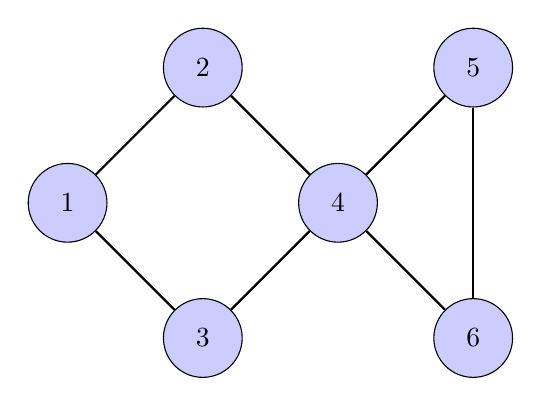
\begin{tikzpicture}
        \node[main node] (1) {1};
        \node[main node] (2) [above right = 1cm and 1cm of 1] {2};
        \node[main node] (3) [below right = 1cm and 1cm of 1] {3};
        \node[main node] (4) [below right = 1cm and 1cm of 2] {4};
        \node[main node] (5) [above right = 1cm and 1cm of 4] {5};
        \node[main node] (6) [below right = 1cm and 1cm of 4] {6};

        \ed12
        \ed13
        \ed43
        \ed42
        \ed45
        \ed46
        \ed56
    \end{tikzpicture}
\end{center}
The best elimination tree you can build looks like this:
\begin{center}
    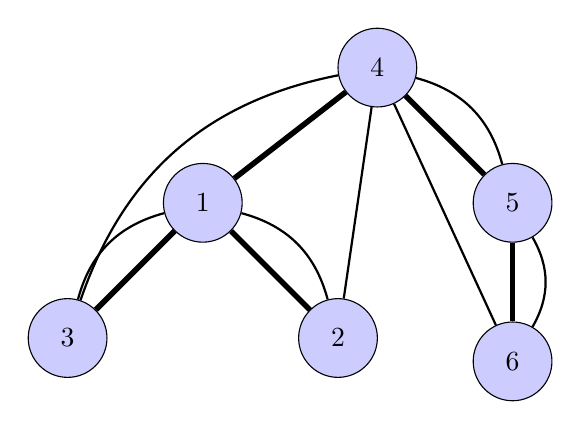
\begin{tikzpicture}
        \node[main node] (4) {4};
        \node[main node] (1) [below left = 1cm and 1.5cm of 4] {1};
        \node[main node] (2) [below right = 1cm and 1cm of 1] {2};
        \node[main node] (3) [below left = 1cm and 1cm of 1] {3};
        \node[main node] (5) [below right = 1cm and 1cm of 4] {5};
        \node[main node] (6) [below = 1cm of 5] {6};

        \ted41
        \ted12
        \ted13
        \ted54
        \ted56

        \edl12
        \edr13
        \edr43
        \ed42
        \edl45
        \ed46
        \edl56
    \end{tikzpicture}
\end{center}
This is not very hard to see: if you pick any other node than 4 as the root for
the elimination tree, then the remaining graph is connected. Hence there cannot
be two subtrees below that root, because there would be edges going between
them. Hence, the tree will start with a root and a single node below it, which
means it will have depth at least 3. Thus we might as well pick a root node 4,
and since the remaining graph is not totally disconnected, the depth of this
tree will be at least 3.

This motivates the following alternative definition.
\begin{definition}
    Let $1$ be the one-vertex graph, and let $\CC(G)$ be the set of connected components of
    the graph $G$. The treedepth $\TD(G)$ of a connected graph $G$ is recursively defined as
    \begin{align*}
        \TD(1) &= 1 \\
        \TD(G) &= 1 + \max_{X \in \CC(G)} \TD(X).
    \end{align*}
\end{definition}
Before we go on to suggest how we do compute this effectively, let us make some
basic observations about treedepth.
\begin{proposition}~
    \begin{enumerate}
        \item Let $L_n$ be the line graph on $n$ nodes. Then $\TD(L_n) =
            \lceil\log_2(n+1)\rceil$.
        \item Let $C_n$ be the cycle graph on $n$ nodes. Then $\TD(C_n) = 1 +
            \lceil\log_2(n)\rceil$.
        \item Let $|G| = n$. Then $\TD(G) = n \iff G = K_n$, the complete graph on $n$
            vertices.
        \item There is an $n \geq 1$ with $G = K_{1,n}$ if and only if $\TD(G) =
            2$.
        \item If $X$ is an induced subgraph of $Y$, then $\TD(X) \leq \TD(Y)$.
    \end{enumerate}
\end{proposition}
We can naively turn the second definition of treedepth into an algorithm. In
this document, I use Python as ``pseudo-code'', but the real code should be C++
for speed. The type \texttt{SubGraph} refers to the fact that $G$ is a subgraph
of the global graph for which we are solving the problem.
\begin{minted}[linenos, frame=leftline]{python}
def treedepth(G : SubGraph) -> int:
    if len(G.vertices()) == 1:
        return 1
    td = len(G.vertices())
    for v in G.vertices():
        G_v = G.without_vertex(v)
        cur_td = 0
        for H in G_v.connected_components():
            cur_td = max(cur_td, 1 + tree_depth(H))
        td = min(td, cur_td)
    return td
\end{minted}
I propose we use \emph{essentially} the algorithm above. However, we
aggressively prune the search tree, and traverse it heuristically instead of
randomly.

In general, it appears that the heuristic strategy for building a tree that witnesses
low treedepth is: choose a root node that breaks up the graph as much as possible. Ideally it
will actually split the graph into pieces that are as light\footnote{I'm going to use
\emph{light} to informally mean ``low treedepth'' and \emph{heavy} correspondingly} as
possible, but if there is no node that even splits the graph up at all you may want to look at
a node so that removing that node creates a node that makes the graph splittable, or just any
node with high \emph{centrality} (for whatever definition of centrality you use). 

I propose the following algorithm template.
\begin{minted}[linenos, frame=leftline]{python}
def treedepth(G : SubGraph, search_lbnd : int, search_ubnd : int) -> (int, int):
    """
    returns (lower, upper): a lower and an upper bound on the
    treedepth of subgraph G.

    search_lbnd: A sister branch provably has depth at least search_lbnd, so
    there is no need to try to prove that this subgraph has depth < search_lbnd
    (on this iteration).

    search_ubnd: If the this subgraph has treedepth >= search_ubnd then we can
    stop with this branch, because there already exists a better solution.
    """
    if search_ubnd <= 1 or search_lbnd >= len(G.vertices()):
        cache.add(G, 1, len(G.vertices())
        return 1, len(G.vertices())
  
    # The cache checks previously checked subgraphs. A lower bound for a
    # superset is also a lower bound for G, and vice versa. One major
    # programming effort will be a smart data structure that makes these
    # operations fast. (e.g., SetTrie + a hashmap for exact matches)
    lower = cache.get_upper_bound_of_subsets(G)
    upper = cache.get_lower_bound_of_supersets(G)

    if search_ubnd <= lower or search_lbnd >= upper or lower == upper:
        cache.add(G, lower, upper)
        return lower, upper

    # exact_methods contains fast methods for exactly determining the treedepth
    # of a graph. For example, they check if the graph is a line graph, cycle,
    # star, or clique. They return the exact treedepth in that case and None
    # otherwise.
    for method in exact_methods:
        exact_td = method(G)
        if exact_td:
            cache.add(G, exact_td, exact_td)
            return exact_td
    
    # heuristic_methods contains methods that heuristically try to find bounds
    # (both lower and upper) on the treedepth of a graph. The bounds are exact,
    # but they may not be tight.
    for method in heuristic_methods:
        heur_lower, heur_upper = method(G)
        lower, upper = min(lower, heur_lower), max(upper, heur_upper)
        if search_ubnd <= lower or search_lbnd >= upper or lower == upper:
            cache.add(G, lower, upper)
            return lower, upper

    # We cannot use easy methods, so we need to recur a level deeper. First, we
    # sort the vertices by centrality -- these are most likely to give us good
    # bounds.
    vertex_order = sorted(G.vertices(), key=lambda v : G.centrality(v),
        reverse=True)

    # Variable to keep track of whether or not this recursion gives us a new
    # lower bound: this happens only if *every* choice of v gives us at least
    # one connected component with a high lower bound.
    new_lower = 0

    for v in vertex_order:
        G_v = G.without_vertex(v)

        # The initial search bounds for G_v. Note that the search_lbnd_v is
        # fixed at search_lbnd - 1, so no need to make a variable.
        search_ubnd_v = min(search_ubnd - 1, upper - 1)

        # The new bounds we get from this choice of v.
        upper_from_v = 0
        lower_from_v = lower

        for H in G_v.connected_components():
            lower_H, upper_H = treedepth(X, search_lbnd - 1, search_ubnd_v)

            # Have we proved that this v will not improve our score (further)?
            if lower_H >= search_ubnd_v:
                break

            upper_from_v = max(upper_from_v, upper_H)
            lower_from_v = min(lower_from_v, lower_H)

            search_lbnd_v = max(search_lbnd_v, lower_H)

        new_lower = max(new_lower, lower_from_v)
        upper = min(upper, upper_from_v)

        # Early exit: this choice of v was either as good as was useful in this
        # branch, or provably optimal for this branch.
        if search_lbnd >= upper or lower == upper:
            cache.add(G, lower, upper)
            return lower, upper

    lower = min(lower, new_lower)

    cache.add(G, lower, upper)
    return lower, upper
\end{minted}
There are two important things missing from this algorithm, one technical and
one conceptual.

The technical thing that is missing is that we currently do not store the
optimal way to actually reconstruct the elemination tree that witnesses the
treedepth of G. This is a matter of caching that construction effectively (e.g.
storing the instructions also in the cache).

The conceptual thing is that the algorithm scaffold currently does not
incorporate any kind of \emph{search depth}. Once the algorithm is recursively
called for the first time, on $G\setminus \{v\}$ for a heuristically chosen $v$,
it will exhaust this branch in its entirety before trying out another $G
\setminus \{w\}$. If it turns out that $v$ was a sub-optimal choice, and
furthermore this would have been easy to find out (by a good upper bound) when
traversing the search tree for $G \setminus \{w\}$, we waste a lot of time. We
would ameliorate this problem, by, say, searching $G \setminus \{v\}$
superficially (for each $v$), and only when that is done, thoroughly searching
$G \setminus \{v\}$ with the bounds found in the superficial search.

Here is a simple way to implement something of this sort: we introduce an
additionaly parameter \texttt{search\_depth} to the algorithm. If
$\mathtt{search\_depth} = 0$, we skip the recursive step at the end, and just
return \texttt{lower, upper} as they are then. In the recursive step, we call
the algorithm with a new \texttt{search\_depth} of \texttt{search\_depth - 1}.

Then the top-level call to the algorithm becomes something like the following.

\begin{minted}[linenos, frame=leftline]{python}
for search_depth in len(G.vertices()):
    lower, upper = treedepth(G, 1, len(G.vertices()), search_depth)
    if lower == upper:
        break
\end{minted}

This is, however, not very sophisticated: if a node has \emph{really} low
centrality you probably do not want to do even a superficial search until you
have done a thorough search of promising nodes first.
\end{document}
